\documentclass{article}

\usepackage[a4paper]{geometry}
\usepackage[ngerman]{babel}
\usepackage[utf8]{inputenc}
\usepackage[T1]{fontenc}
\usepackage{tabularx}
\usepackage{hyperref}
\usepackage{graphicx}

\graphicspath{{./diagrams/}}

\hypersetup{colorlinks=true, linkcolor=black, filecolor=black, urlcolor=black}

\begin{document}

\begin{titlepage}
	\begin{flushleft}
		TH Brandenburg \\
		Online Studiengang Medieninformatik \\
		Fachbereich Informatik und Medien \\
		Softwaretechnik \\
		Prof. Dr-Ing. Martin Schafföner
	\end{flushleft}

	\vfill

	\begin{center}
		\Large{Einsendeaufgabe 2: UML}\\[0.5em]
		\large{Sommersemester 2021}\\[0.25em]
		\large{Abgabetermin 10.06.2021}
	\end{center}

	\vfill

	\begin{flushright}
		Mara Schulke \\
		Matrikel-Nr. 20215853
	\end{flushright}
\end{titlepage}

\tableofcontents

\vfill

\section{Aufgabenstellung}

Im Moodle-Kurs wurde folgende Aufgabenstellung bekannt gegeben:

\begin{quote}
	Die Aufgabenstellung benötigt Ihre bisherigen Ergebnisse aus der ESA1.
	Bitte entwerfen Sie für Ihre in ESA1 entworfene Problemstellung zwei
	verschiedene UML-Diagramme, die sich jeweils an verschiede
	Interessenvertreter bzw. Projektteilnehmer richten sollen. Die Lösung MUSS
	ein Klassendiagramm und ein Aktivitätsdiagramm enthalten. Begründen Sie,
	welches weitere UML-Diagramm sie als nächstes erstellen würden. Beim
	Klassendiagramm können Sie auf die detaillierte Darstellung von Methoden
	verzichten, wichtige Attribute sollen jedoch enthalten sein. Achten Sie auf
	richtige Verwendung von Assoziation, Aggregation und Komposition sowie auf
	Multiplizitäten.
\end{quote}

\newpage

\section{Klassendiagramm}

\vfill

\begin{figure}[h]
	\centering
	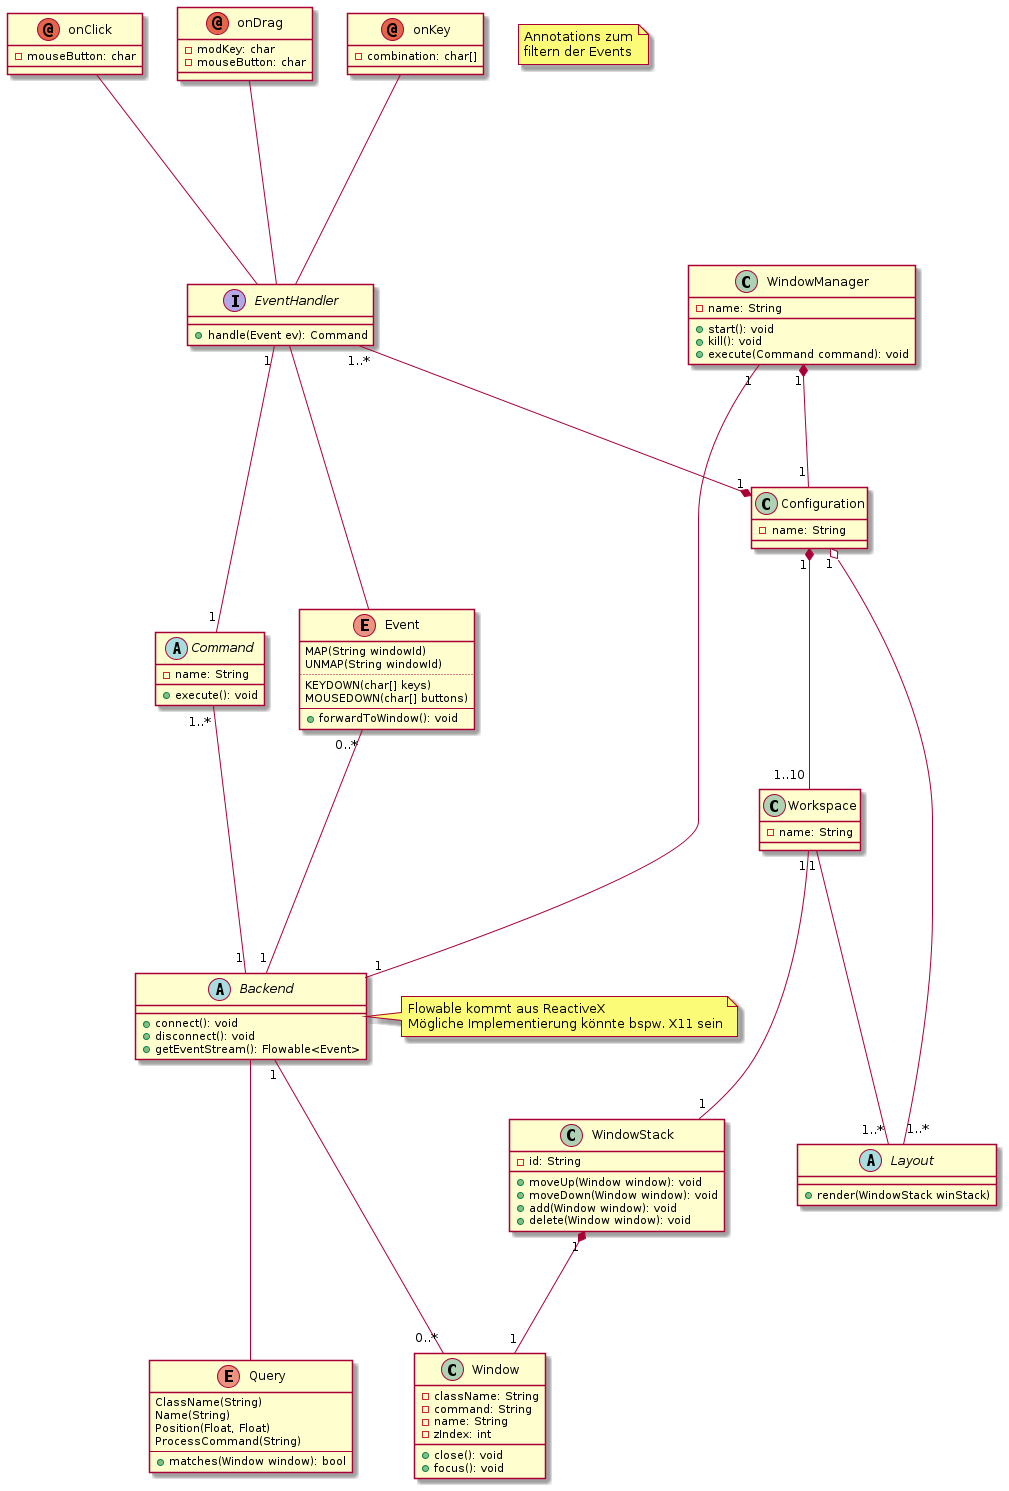
\includegraphics[width=0.55\textwidth]{class}
	\caption{Klassendiagramm}
\end{figure}

\vfill

Dieses Klassendiagramm könnte eine gute Dokumentationsgrundlage darstellen und
einem Konfigurierenden einen guten Überblick über die grobe Struktur der
Software und die Rolle seiner Konfiguration geben.

\newpage

\section{Aktivitätsdiagramm}

\vfill

\begin{figure}[h]
	\centering
	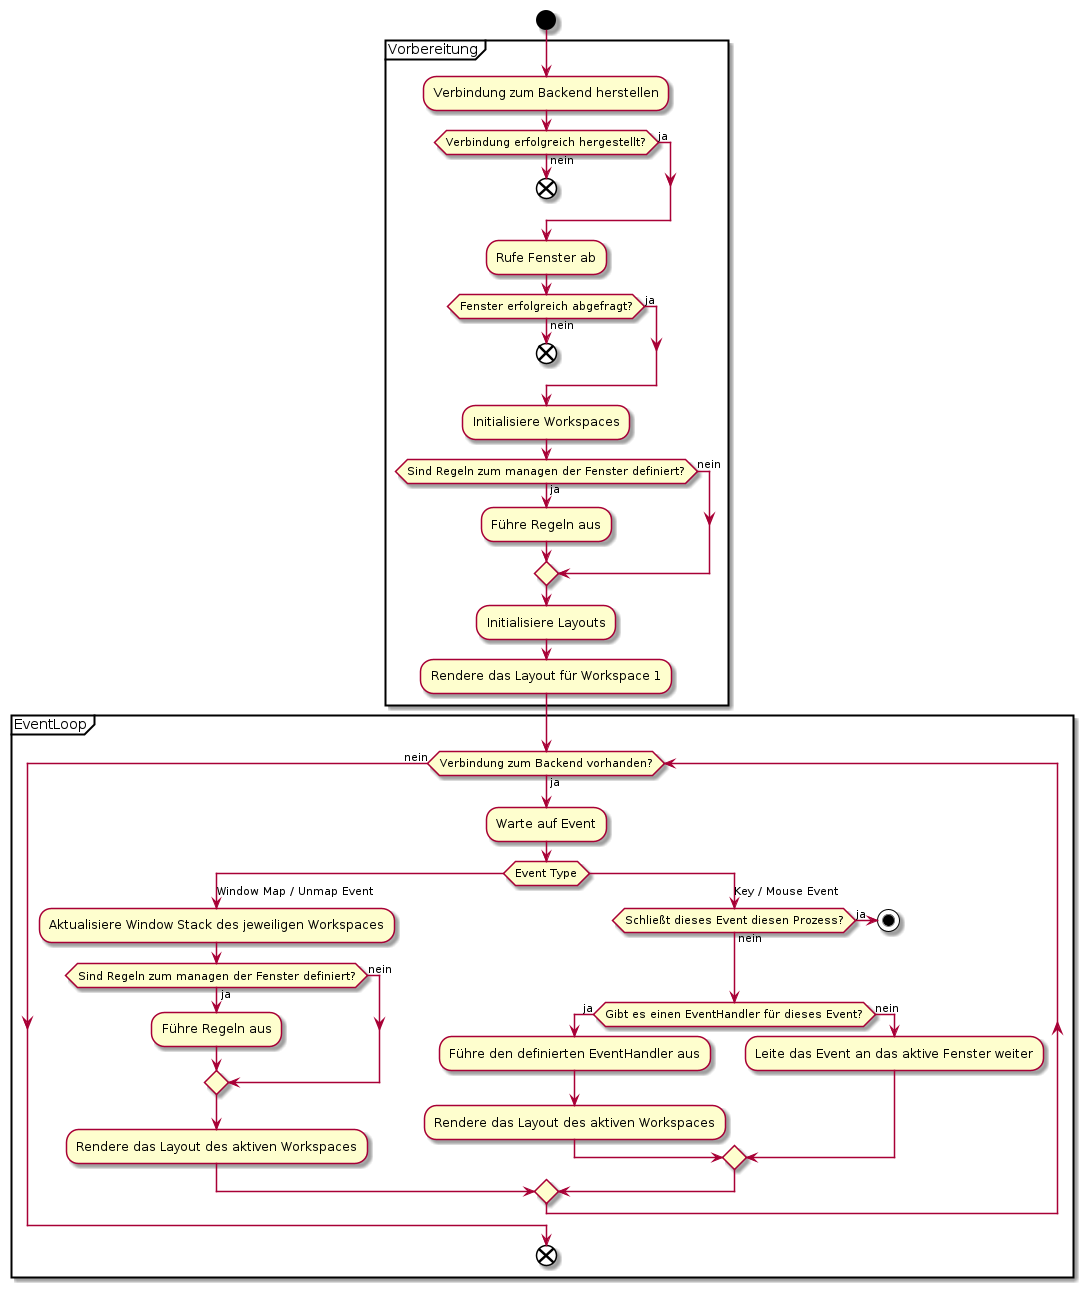
\includegraphics[height=0.7\textheight]{activity}
	\caption{Aktivitätsdiagramm}
\end{figure}

\vfill

Durch dieses Aktivitätsdiagramm können Entwickler eine Übersicht über den
Ablauf des Main-Threads des Window Managers erhalten und dies als Gundlage
für eine Implementierung verwenden.

\section{Empfehlung für ein weiteres Diagramm}

Als weiteres Diagramm könnte ein Paketdiagramm interessant sein, da dies für
die Entwickler und die Konfigurierenden einen Mehrwert bietet.

\end{document}
